\documentclass{beamer}
\setbeamertemplate{navigation symbols}{}

\usepackage{beamerthemeshadow}
\setbeamertemplate{caption}[numbered]

\hypersetup{colorlinks}

\def\gw#1{gravitational wave#1 (GW#1)\gdef\gw{GW}}
\def\ns#1{neutron star#1 (NS#1)\gdef\ns{NS}}

\newcommand{\red}[1]{{\color{red}{#1}}}

\begin{document}

\begin{frame}
    \frametitle{James A. Clark: Gravitational Wave Data Analysis}

    \begin{columns}[]
        \column{0.6\textwidth}
        \begin{center}

            \begin{small}
                \begin{itemize}
                    \item 
                \end{itemize}
            \end{small}

    \begin{center}
        \vspace{-0.75cm}
        \begin{figure}
            \scalebox{0.35}{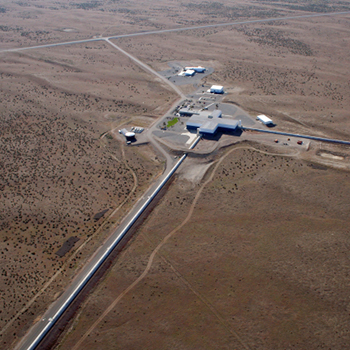
\includegraphics{lho4s.jpg}} \\
        \end{figure}
    \end{center}

    \end{center}


        \column{0.5\textwidth}

    \begin{center}
        \vspace{-0.75cm}
        \begin{figure}
            \scalebox{0.35}{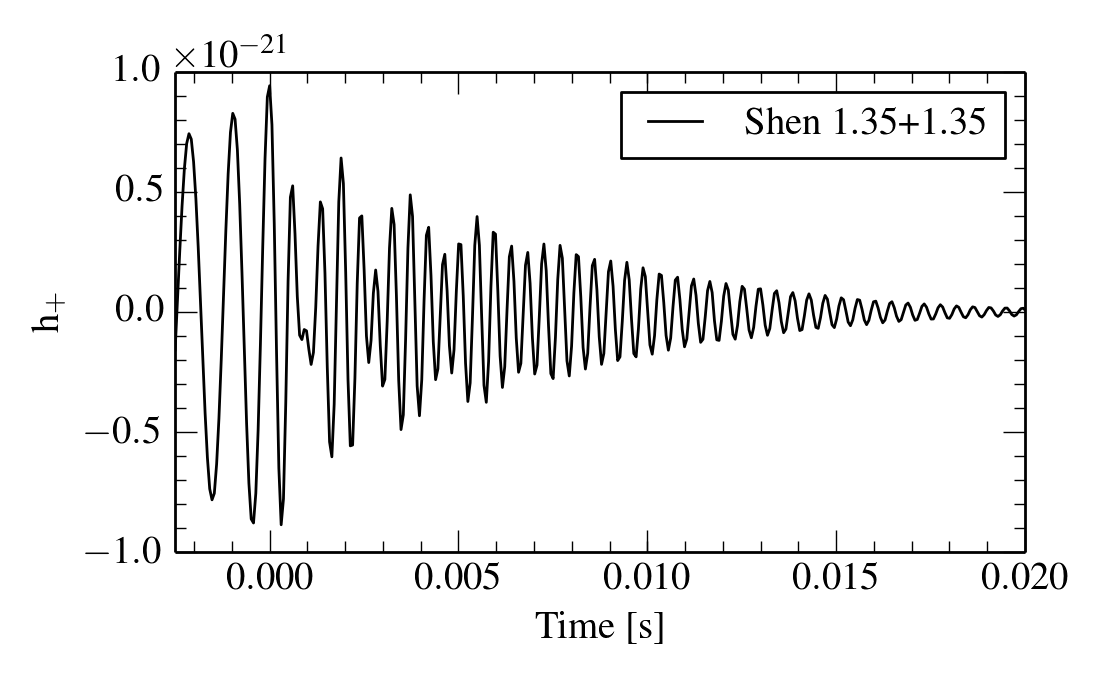
\includegraphics{pmns_example.png}} \\
            \scalebox{0.25}{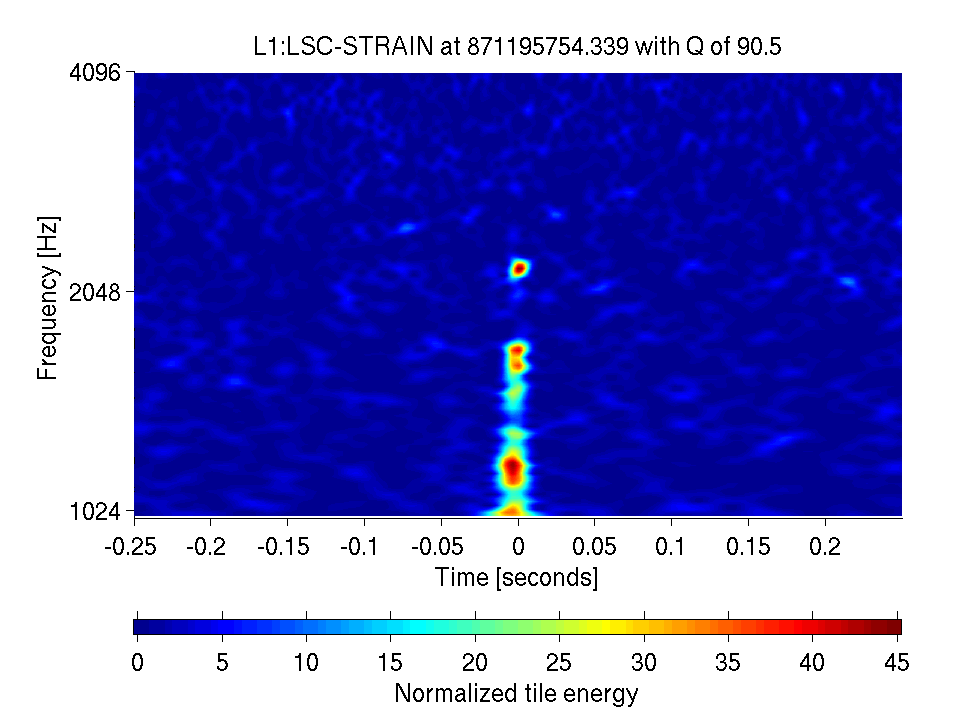
\includegraphics{pmns_tfmap.png}}
        \end{figure}
    \end{center}

    \end{columns}


\end{frame}





\end{document}
